%% 6章用 (Comparison)

以下の図表は，グリッド極値点探索法とBrent法の性能を比較したものである（対象関数: $f(x) = \frac{1}{1+25x^2}$，次数: $n=15$）．

表\ref{tab:remes-comparison-summary}は，両手法の収束性能，計算時間，最終精度を比較した総合評価である．
Brent法は計算時間がやや増加するものの，極値探索精度の向上により，より高精度な最良近似多項式が得られることが示されている．

図\ref{fig:remes-comparison-deviation}は，各極値点における理論値からの偏差を可視化したものである．
グリッド極値点探索では離散化誤差により微小なズレが残るのに対し，Brent法では機械イプシロンレベルの精度が達成されている．

\begin{figure}[H]
 \centering
 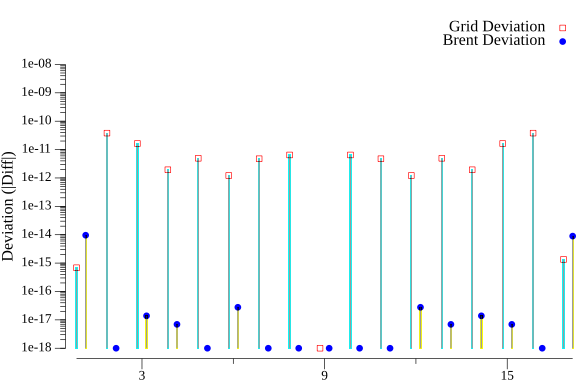
\includegraphics[width=0.8\linewidth]{material/remes/outputs/comparison/deviation_comparison.png}
 \caption{極値点ごとの理論値からの偏差 ($|\text{Calc} - \text{True}|$)}
 \label{fig:remes-comparison-deviation}
\end{figure}

\begin{table}[H]
 \centering
 \caption{グリッド法とBrent法の性能比較概要 ($n=15$)}
 \label{tab:remes-comparison-summary}
 \begin{tabular}{lcccc}
 \toprule
 手法 & 反復回数 & 収束判定値 & 高精度な最大誤差 $\|E\|$ & 計算時間 \\
 \midrule
 Grid Search & 6 & $6.10623e-16$ & $2.97811e-02$ & 268.04403ms \\
 Brent Method & 20 & $4.44089e-16$ & $2.97767e-02$ & 796.27914ms \\
 \bottomrule
 \end{tabular}
\vspace{1mm}

\footnotesize\textbf{高精度な最大誤差について：}
区間 $[-1.0,1.0]$ を50,000個の格子点で均等分割し，誤差関数 $|E(x)|$ の局所極大値を検出した後，
各極大値の近傍に対してBrent法を適用して算出した値である．
\end{table}

\begin{table}[H]
 \centering
 \caption{各極値点における真の誤差との偏差比較（等振幅性の崩れ）}
 \label{tab:remes-comparison-detail}
 \begin{tabular}{crrr}
 \toprule
 No. & Grid偏差 ($|\Delta E|$) & Brent偏差 ($|\Delta E|$) & 精度比 (Grid/Brent) \\
 \midrule
 1 & $6.86950e-16$ & $9.60343e-15$ & $0.1$ \\
 2 & $3.80066e-11$ & $0.00000e+00$ & $0.0$ \\
 3 & $1.63316e-11$ & $1.38778e-17$ & $1176819.0$ \\
 4 & $1.94925e-12$ & $6.93889e-18$ & $280916.0$ \\
 5 & $4.93021e-12$ & $0.00000e+00$ & $0.0$ \\
 6 & $1.21936e-12$ & $2.77556e-17$ & $43932.0$ \\
 7 & $4.76352e-12$ & $0.00000e+00$ & $0.0$ \\
 8 & $6.46216e-12$ & $0.00000e+00$ & $0.0$ \\
 9 & $0.00000e+00$ & $0.00000e+00$ & $0.0$ \\
 10 & $6.46216e-12$ & $0.00000e+00$ & $0.0$ \\
 11 & $4.76358e-12$ & $0.00000e+00$ & $0.0$ \\
 12 & $1.21927e-12$ & $2.77556e-17$ & $43929.0$ \\
 13 & $4.93020e-12$ & $6.93889e-18$ & $710517.0$ \\
 14 & $1.94927e-12$ & $1.38778e-17$ & $140459.5$ \\
 15 & $1.63316e-11$ & $6.93889e-18$ & $2353638.0$ \\
 16 & $3.80066e-11$ & $0.00000e+00$ & $0.0$ \\
 17 & $1.34615e-15$ & $8.93036e-15$ & $0.2$ \\
 \bottomrule
 \end{tabular}
\end{table}

\noindent\textbf{考察:}
表\ref{tab:remes-comparison-summary}において，全区間を対象とした高精度な再評価を行った結果，
Grid法の最大誤差 $\|E\|$ は $2.978113e-02$ となり，Brent法の $2.977669e-02$ よりも大きな値を示した．
これは，Grid法が離散的な探索により真の最大誤差（ピーク）を取りこぼして収束していたことを示唆しており，
Brent法を用いることで，より最大誤差が小さく，最良近似多項式に近い結果が得られたことを裏付けている．
また，表\ref{tab:remes-comparison-detail}に示すように，各極値点における等振幅性の偏差はBrent法の方が平均して約 7905 倍小さく，
数学的性質の観点からもBrent法がより高精度な近似解を得られていることが確認できる．
